% concatenated from main_geomtric__2_.tex
\documentclass[
  aip,
  amsmath,amssymb,
  preprint
]{revtex4-1}

\usepackage{graphicx}
\usepackage{amsmath,amssymb,amsthm}
\usepackage{booktabs}
\usepackage{array}
\usepackage{enumitem}
\usepackage{tikz}
\usetikzlibrary{patterns,calc,arrows.meta}
\usepackage{algpseudocode}
\usepackage{url} % optional but safe
\usepackage{enumitem}

% Keep hyperref last
\usepackage{hyperref}

% Theorems
\newtheorem{theorem}{Theorem}[section]
\newtheorem{lemma}[theorem]{Lemma}
\newtheorem{proposition}[theorem]{Proposition}
\newtheorem{corollary}[theorem]{Corollary}
\newtheorem{remark}{Remark}[section]
\newtheorem{definition}{Definition}[section]


\begin{document}
\raggedbottom


\title{Group-Theoretical Origin of the Sectoral-Tesseral-Zonal Trichotomy in Spherical Harmonics}

\author{Mustafa Bakr}
\email{mustafa.bakr@physics.ox.ac.uk}
\affiliation{Clarendon Laboratory, Department of Physics, University of Oxford}
\author{Smain Amari}
%\date{\today}


\begin{abstract}
The spherical harmonics $Y_\ell^m$ fall into three families---sectoral ($\ell = |m|$), tesseral ($\ell > |m| > 0$), and zonal ($m = 0$)---which exhibit fundamentally different behaviour under analytic continuation to non-integer parameters. We demonstrate that this trichotomy has a natural explanation in the representation theory of SO(3). Sectoral harmonics correspond to highest-weight vectors annihilated by the raising operator $L_+$; this annihilation condition reduces to a first-order differential equation admitting solutions for any real $m > 0$, independent of representation-theoretic constraints. Tesseral harmonics arise from the full ladder algebra acting on highest-weight states; for non-integer $m$, this construction yields tesseral modes at $\nu = m + k$ for positive integer $k$, with the hypergeometric series terminating when $\nu - m$ is a non-negative integer. Zonal harmonics with $m = 0$ require integer $\nu$ on the full sphere, but TE-polarised zonal modes survive in wedge geometries because their electric field components automatically satisfy the conducting boundary conditions. Numerical simulations of electromagnetic cavities with conducting wedges confirm these predictions quantitatively: both sectoral modes ($\nu = m$) and tesseral modes ($\nu = m + k$) are observed with sub-percent frequency agreement, validating the extended framework for non-integer azimuthal index.
\end{abstract}



\maketitle


\section{Introduction}

The spherical harmonics $Y_\ell^m(\theta, \phi)$ provide the angular eigenfunctions for the Laplacian on the sphere and appear throughout mathematical physics. Their applications range from the quantum theory of angular momentum, as developed by Wigner~\cite{Wigner1959} and exposited in the standard treatments of Rose~\cite{Rose1957} and Edmonds~\cite{Edmonds1957}, to electromagnetic cavity modes in classical electrodynamics~\cite{Stratton1941,Jackson1999}. For problems posed on the full sphere with standard boundary conditions, the indices are restricted to non-negative integers $\ell = 0, 1, 2, \ldots$ with $|m| \leq \ell$. This quantisation is conventionally attributed to regularity requirements at the poles, a viewpoint developed rigorously in the treatises on special functions by Whittaker and Watson~\cite{WhittakerWatson1927} and Hobson~\cite{Hobson1931}.

Recent work on electromagnetic cavities with modified boundaries has revealed that the three traditional families of spherical harmonics---sectoral, tesseral, and zonal---behave fundamentally differently under continuation to non-integer parameters~\cite{BakrAmari2025, bakrsphere, bakr2025quantummechanicssphericalwedge, bakr2025zerofrequency}. Sectoral modes with $\ell = |m|$ can be extended to continuous real values of $m$, while tesseral and zonal modes cannot. This asymmetry, though derivable from the analytic properties of Legendre functions as catalogued in the Digital Library of Mathematical Functions~\cite{DLMF}, calls for a deeper explanation.

The purpose of this paper is to demonstrate that the sectoral-tesseral-zonal trichotomy originates in the representation theory of the rotation group SO(3), whose general theory is developed in the monographs of Vilenkin~\cite{Vilenkin1968}, Varshalovich, Moskalev, and Khersonskii~\cite{Varshalovich1988}, and from a modern mathematical perspective by Hall~\cite{Hall2015} and Knapp~\cite{Knapp2001}. The key observation is that sectoral harmonics are highest-weight vectors in SO(3) representations, characterised by annihilation under the raising operator $L_+$. This annihilation condition constitutes a first-order differential equation whose solutions exist for any positive real $m$, regardless of whether $m$ is an integer. Tesseral and zonal harmonics, by contrast, are obtained by applying lowering operators to highest-weight vectors, and this construction requires integer $\ell - |m|$ for the representation to close finitely. The integrality constraint for non-sectoral modes is thus a consequence of finite-dimensional unitary representation theory, not merely of polar regularity.

This perspective explains a puzzle arising in the study of electromagnetic cavities with domain modifications. Wedges restricting the azimuthal range~\cite{BakrAmari2023, BakrAmari20251} provide clean access to continuous sectoral modes, while cones truncating the polar domain create fundamentally different boundary-value problems rather than analytic continuations of full-sphere modes. The group-theoretical framework clarifies why: wedges relax the single-valuedness constraint while preserving the highest-weight structure, whereas accessing continuous non-sectoral modes would require abandoning the ladder algebra entirely.

The principal contribution of this work is not the observation that highest-weight states satisfy a first-order differential equation---this is well known from the quantum theory of angular momentum~\cite{Sakurai2017}. Rather, it is the recognition that this first-order structure permits extension to non-integer values of $m$ when the azimuthal domain is restricted, and that the resulting framework provides a complete explanation of the sectoral-tesseral-zonal trichotomy. The distinct continuation properties of the three mode families are not accidents of special function formulas but inevitable consequences of how each family relates to the angular momentum ladder algebra. Since this structure is rooted in the geometry of the sphere, the framework applies universally wherever the angular Laplacian governs wave propagation---from electromagnetic cavities to quantum central potentials to black hole perturbations.

\section{Angular Momentum Algebra and Spherical Harmonics}

The rotation group SO(3) has Lie algebra $\mathfrak{so}(3)$ spanned by the angular momentum operators $L_x$, $L_y$, $L_z$ satisfying the commutation relations
\begin{equation}
[L_i, L_j] = i\varepsilon_{ijk} L_k,
\label{eq:commutation}
\end{equation}
where $\varepsilon_{ijk}$ is the Levi-Civita symbol and we work in units with $\hbar = 1$. The Casimir operator $\mathrm{L}^2 = L_x^2 + L_y^2 + L_z^2$ commutes with all generators and therefore takes a constant value on each irreducible representation. The structure of irreducible representations is most efficiently analysed using the ladder operators $L_\pm = L_x \pm i L_y$, which satisfy $[L_z, L_\pm] = \pm L_\pm$ and $[L_+, L_-] = 2L_z$.

The finite-dimensional irreducible representations of SO(3) are labelled by non-negative integers $\ell = 0, 1, 2, \ldots$, as established in the foundational work of Wigner~\cite{Wigner1959}. The representation $\mathcal{D}^\ell$ has dimension $2\ell + 1$ and is spanned by eigenstates $|\ell, m\rangle$ of $L_z$ with eigenvalues $m = -\ell, -\ell+1, \ldots, \ell-1, \ell$. The Casimir operator acts as $\mathrm{L}^2 |\ell, m\rangle = \ell(\ell+1) |\ell, m\rangle$, and the ladder operators connect adjacent states according to
\begin{equation}
L_\pm |\ell, m\rangle = \sqrt{\ell(\ell+1) - m(m\pm 1)} \, |\ell, m\pm 1\rangle.
\label{eq:ladder_action}
\end{equation}

The state $|\ell, \ell\rangle$ with maximal $L_z$ eigenvalue is called the highest-weight vector of the representation. It is characterised by the property $L_+ |\ell, \ell\rangle = 0$, which follows from equation~\eqref{eq:ladder_action} since the coefficient $\sqrt{\ell(\ell+1) - \ell(\ell+1)}$ vanishes. The entire representation can be generated from this single state by repeated application of the lowering operator: $|\ell, m\rangle \propto (L_-)^{\ell - m} |\ell, \ell\rangle$ for $m = \ell, \ell-1, \ldots, -\ell$. The representation closes after exactly $2\ell$ applications of $L_-$, when $L_- |\ell, -\ell\rangle = 0$.

In the coordinate representation on the sphere, the angular momentum operators take the differential form~\cite{Sakurai2017}
\begin{equation}
L_z = -i\frac{\partial}{\partial\phi}, \qquad L_\pm = e^{\pm i\phi}\left(\pm\frac{\partial}{\partial\theta} + i\cot\theta\frac{\partial}{\partial\phi}\right),
\label{eq:differential_form}
\end{equation}
and the Casimir operator becomes the angular Laplacian
\begin{equation}
\mathrm{L}^2 = -\frac{1}{\sin\theta}\frac{\partial}{\partial\theta}\left(\sin\theta\frac{\partial}{\partial\theta}\right) - \frac{1}{\sin^2\theta}\frac{\partial^2}{\partial\phi^2}.
\label{eq:angular_laplacian}
\end{equation}
The spherical harmonics $Y_\ell^m(\theta, \phi)$ are the coordinate-space representatives of the abstract states $|\ell, m\rangle$, providing simultaneous eigenfunctions of $\mathrm{L}^2$ and $L_z$.


\section{The Sectoral Family as Highest-Weight Solutions}

We now arrive at the central observation of this paper. The highest-weight condition $L_+ \psi = 0$, when expressed in coordinate form, reduces to a first-order differential equation whose solutions exist for any positive real value of the weight parameter, independently of whether that parameter is an integer.

Consider a function of the separable form $\psi(\theta, \phi) = f(\theta) e^{im\phi}$, where $m$ is not assumed to be an integer. This function is an eigenstate of $L_z$ with eigenvalue $m$, since $L_z \psi = m\psi$ follows directly from equation~\eqref{eq:differential_form}. Applying the raising operator yields
\begin{equation}
L_+ \psi = e^{i(m+1)\phi}\left(f'(\theta) - m\cot\theta \cdot f(\theta)\right),
\label{eq:raising_applied}
\end{equation}
as may be verified by straightforward calculation. The highest-weight condition $L_+ \psi = 0$ therefore requires
\begin{equation}
f'(\theta) = m\cot\theta \cdot f(\theta).
\label{eq:first_order}
\end{equation}

This is a separable first-order ordinary differential equation. Writing $df/f = m\cot\theta \, d\theta = m \, d(\ln\sin\theta)$ and integrating, one obtains $\ln|f| = m\ln|\sin\theta| + \text{const}$, hence
\begin{equation}
f(\theta) = C(\sin\theta)^m
\label{eq:sectoral_solution}
\end{equation}
for an arbitrary constant $C$. The solution exists and is unique (up to normalisation) for any real $m$. For $m > 0$, the function $(\sin\theta)^m$ vanishes at both poles as $\theta^m$ near $\theta = 0$ and $(\pi-\theta)^m$ near $\theta = \pi$, ensuring regularity on the entire sphere.

\begin{theorem}[Continuous Sectoral Family]
\label{thm:sectoral}
The function
\begin{equation}
\psi_m(\theta, \phi) = (\sin\theta)^m e^{im\phi}
\label{eq:full_sectoral}
\end{equation}
satisfies $L_+ \psi_m = 0$ and $L_z \psi_m = m\psi_m$ for any real $m > 0$, and is regular at both poles of the sphere. The Casimir eigenvalue is $\mathrm{L}^2 \psi_m = m(m+1)\psi_m$.
\end{theorem}

\begin{proof}
The properties $L_+ \psi_m = 0$ and $L_z \psi_m = m\psi_m$ follow from the construction above. For the Casimir eigenvalue, we use the identity $\mathrm{L}^2 = L_- L_+ + L_z^2 + L_z$, which follows from the commutation relations. Applying this to a state annihilated by $L_+$ gives $\mathrm{L}^2 \psi_m = (L_z^2 + L_z)\psi_m = (m^2 + m)\psi_m = m(m+1)\psi_m$. Regularity at the poles follows from the behaviour $(\sin\theta)^m \to 0$ as $\theta \to 0$ or $\theta \to \pi$ for $m > 0$.
\end{proof}

\begin{remark}[Domain of validity]
\label{rem:domain}
For non-integer $m$, the function $\psi_m$ is multi-valued on the full sphere and does not belong to $L^2(S^2)$. The relations $L_+ \psi_m = 0$, $L_z \psi_m = m\psi_m$, and $\mathbf{L}^2 \psi_m = m(m+1)\psi_m$ hold as differential identities, but $\psi_m$ is not an eigenstate in the spectral-theoretic sense until the domain is restricted to a simply connected region (such as a wedge) where single-valuedness is not required.
\end{remark}

The fact that highest-weight states satisfy the first-order condition $L_+ \psi = 0$ is well established in the quantum theory of angular momentum~\cite{Sakurai2017}. What has not been emphasised in this context is that the resulting differential equation~\eqref{eq:first_order} admits solutions for any real $m > 0$, not merely for positive integers. The solution $(\sin\theta)^m e^{im\phi}$ exists mathematically for $m = 1.5$ just as surely as for $m = 2$. However, an important distinction must be drawn. For non-integer $m$, the azimuthal factor $e^{im\phi}$ is multi-valued under $\phi \to \phi + 2\pi$, and such functions do not belong to the Hilbert space $L^2(S^2)$ of square-integrable functions on the full sphere. They satisfy the differential relation $L_z \psi = m\psi$ but are not eigenstates of $L_z$ in the spectral-theoretic sense. The integer values $m = 1, 2, 3, \ldots$ appearing in standard treatments are selected precisely by the requirement of single-valuedness.

These non-integer solutions become physically relevant when the azimuthal domain is restricted. A conducting wedge spanning $\phi \in [0, \Phi]$ replaces the periodicity condition with boundary conditions at the wedge faces, and single-valuedness is no longer required. In this context, the functions $(\sin\theta)^m e^{im\phi}$ with $m = n\pi/\Phi$ are valid eigenfunctions of the restricted problem, and the continuous family of sectoral solutions acquires direct physical meaning.

\begin{remark}[The boundary at $m \to 0^+$]
\label{rem:m_zero}
As $m \to 0^+$, the sectoral function $(\sin\theta)^m \to 1$, recovering the  constant function. This limit is annihilated by $L_+$ trivially: applying equation~\eqref{eq:raising_applied} with $f(\theta) = 1$ gives $f'(\theta) = 0$ and $m\cot\theta \cdot f = 0$, so the annihilation condition is satisfied vacuously. The Casimir eigenvalue $m(m+1) \to 0$ in this limit. 

However, this boundary point has a subtle status. While the angular eigenfunction remains well-defined, the electromagnetic fields extracted from it via the Debye potential formalism vanish identically~\cite{BakrAmari2025}. The factor $\nu(\nu+1) = m(m+1)$ that appears in the radial field component vanishes, and the angular derivatives acting on the constant function $(\sin\theta)^0 = 1$ also vanish, eliminating all tangential components. The $m = 0$ boundary thus represents a transition from propagating modes to null field configurations.
\end{remark}

\section{Tesseral and Zonal Modes from the Ladder Construction}
The situation changes fundamentally when we consider spherical harmonics with $\ell > |m|$. These tesseral modes (when $m \neq 0$) and zonal modes (when $m = 0$) cannot be obtained from a first-order equation. They arise instead from the ladder construction
\begin{equation}
Y_\ell^m \propto (L_-)^{\ell - m} Y_\ell^\ell,
\label{eq:ladder_construction}
\end{equation}
which generates lower-weight states from the highest-weight vector by repeated application of the lowering operator.

To understand why this construction requires integer $\ell$, consider what happens when we apply $L_-$ to the sectoral function. A direct calculation using equation~\eqref{eq:differential_form} yields
\begin{equation}
L_- \psi_m = -2m\cos\theta \cdot (\sin\theta)^{m-1} e^{i(m-1)\phi}.
\label{eq:lowering_sectoral}
\end{equation}
This is a new function with $L_z$ eigenvalue $m-1$, as expected. Repeated application generates a sequence of functions with decreasing $L_z$ eigenvalues. The representation closes when the lowering operator annihilates a state, which occurs when the coefficient in equation~\eqref{eq:ladder_action} vanishes. This happens at $m = -\ell$, giving the condition $\ell(\ell+1) = (-\ell)((-\ell)-1) = \ell(\ell+1)$, which is satisfied. The chain of states thus runs from $m = \ell$ down to $m = -\ell$, comprising exactly $2\ell + 1$ states.

\begin{theorem}[Integrality Requirement]
\label{thm:integrality}
The ladder construction~\eqref{eq:ladder_construction} produces a finite set of $2\ell + 1$ linearly independent eigenfunctions of $\mathrm{L}^2$ with eigenvalue $\ell(\ell+1)$ if and only if $\ell$ is a non-negative integer.
\end{theorem}

\begin{proof}
For the chain of states to close, the lowering operator must eventually annihilate a state. Starting from the highest-weight state with $L_z$ eigenvalue $\ell$ and applying $L_-$ repeatedly, the $L_z$ eigenvalue decreases by one at each step: $\ell, \ell-1, \ell-2, \ldots$ The chain terminates when we reach a state with eigenvalue $-\ell$, which requires traversing exactly $2\ell$ steps. For this to yield a finite number of states, $2\ell$ must be a non-negative integer. The further requirement that the representation be single-valued under rotations by $2\pi$---that is, a true representation of SO(3) rather than its double cover SU(2)---restricts $\ell$ to integer values.
\end{proof}

The zonal harmonics with $m = 0$ provide the clearest illustration. To reach $m = 0$ from the highest-weight state $Y_\ell^\ell$, we must apply $L_-$ exactly $\ell$ times:
\begin{equation}
Y_\ell^0 \propto (L_-)^\ell Y_\ell^\ell.
\label{eq:zonal_construction}
\end{equation}
This construction manifestly requires $\ell$ to be a non-negative integer; for non-integer $\ell$, the expression $(L_-)^\ell$ is not even defined within the standard algebraic framework.


\subsection{Analytical Confirmation: Singularity Structure}
\label{subsec:singularity}
The representation-theoretic argument above can be complemented by direct analysis of the associated Legendre equation. Consider a solution $P_\nu^m(\cos\theta)$ that is regular at the north pole $\theta = 0$. Its behavior at the south pole $\theta = \pi$ is determined by hypergeometric connection formulas, which express the solution near one singular point as a linear combination of the two local solutions near the other. The connection formulas, derived in detail in Ref.~\cite{BakrAmari2025}, show that a solution regular at $\theta = 0$ acquires a singular component at $\theta = \pi$ with coefficient proportional to $\sin(\nu\pi)$. This coefficient vanishes if and only if $\nu$ is an integer.

For the sectoral case $\nu = m$, however, the explicit closed-form solution $(\sin\theta)^m$ is manifestly regular at both poles for any real $m > 0$---no connection formula analysis is required. The function vanishes as $\theta^m$ near $\theta = 0$ and as $(\pi - \theta)^m$ near $\theta = \pi$, with no singular component present.

\begin{proposition}[Singularity Dichotomy]
\label{prop:singularity}
Let $\Theta(\theta)$ be a solution of the associated Legendre equation that is
regular at $\theta = 0$.
\begin{enumerate}
\renewcommand{\theenumi}{\roman{enumi}}
\renewcommand{\labelenumi}{(\theenumi)}
\item If $\nu = m$ (sectoral), then $\Theta(\theta) = (\sin\theta)^m$ is regular at
both poles for any real $m>0$.
\item If $\nu \neq m$ (tesseral or zonal), then $\Theta(\theta)$ is regular at $\theta=\pi$
if and only if $\nu - |m|$ is a non-negative integer (equivalently, $\nu = |m| + k$
for some $k \in \mathbb{Z}_{\ge 0}$).
\end{enumerate}
\end{proposition}
This analytical result provides independent confirmation of the representation-theoretic conclusion: non-integer values of $\nu$ produce functions singular at the south pole, which cannot represent physical modes on the full sphere.

\begin{remark}[Algebraic versus analytical perspectives]
\label{rem:perspectives}
The integrality requirement for tesseral and zonal modes emerges from two complementary viewpoints. The algebraic perspective shows that the ladder construction $(L_-)^{\ell-m}$ requires an integer exponent to be well-defined within the representation-theoretic framework. The analytical perspective shows that non-integer $\nu \neq m$ produces solutions with $\sin(\nu\pi) \neq 0$ in the connection formula, generating a singularity at the south pole. 

These viewpoints are not independent but reflect the same underlying structure: the ladder algebra provides an algebraic encoding of the global regularity conditions that the differential equation must satisfy. The singularity arises precisely because the analytic continuation of the ladder construction to non-integer $\ell - m$ fails to produce globally regular functions.

For the sectoral family alone, the first-order annihilation condition $L_+ \psi = 0$ bypasses the ladder construction entirely, yielding a closed-form solution $(\sin\theta)^m$ that is manifestly regular for all real $m > 0$. This is why sectoral modes---and only sectoral modes---admit continuous extension to non-integer parameters on the full sphere.
\end{remark}


\section{The Trichotomy Explained}
We are now in a position to state the complete group-theoretical explanation for the three families of spherical harmonics and their distinct continuation properties.

\begin{theorem}[Group-Theoretical Classification]
\label{thm:classification}
The spherical harmonics $Y_\ell^m$ fall into three families whose distinct behaviour under continuation to non-integer parameters reflects their different relationships to the SO(3) ladder algebra.

The sectoral harmonics with $\ell = |m|$ are highest-weight vectors (or, for negative $m$, lowest-weight vectors) satisfying the first-order annihilation condition $L_+ \psi = 0$. The general solution $(\sin\theta)^{|m|} e^{\pm i|m|\phi}$ exists for any real $|m| > 0$ and is regular on the sphere. The requirement of integer $|m|$ arises solely from azimuthal single-valuedness, not from any intrinsic property of the differential equation.

The tesseral harmonics with $\ell > |m| > 0$ are obtained by applying $(L_\mp)^{\ell - |m|}$ to sectoral modes. This construction requires $\ell - |m|$ to be a positive integer for the representation to have well-defined dimension. No continuous family of tesseral harmonics exists.

The zonal harmonics with $m = 0$ are obtained by applying $(L_-)^\ell$ to the highest-weight state. This construction requires $\ell$ to be a positive integer. The only continuous zonal solution is the trivial constant function at $\ell = 0$.
\end{theorem}

\begin{figure}[t]
\centering
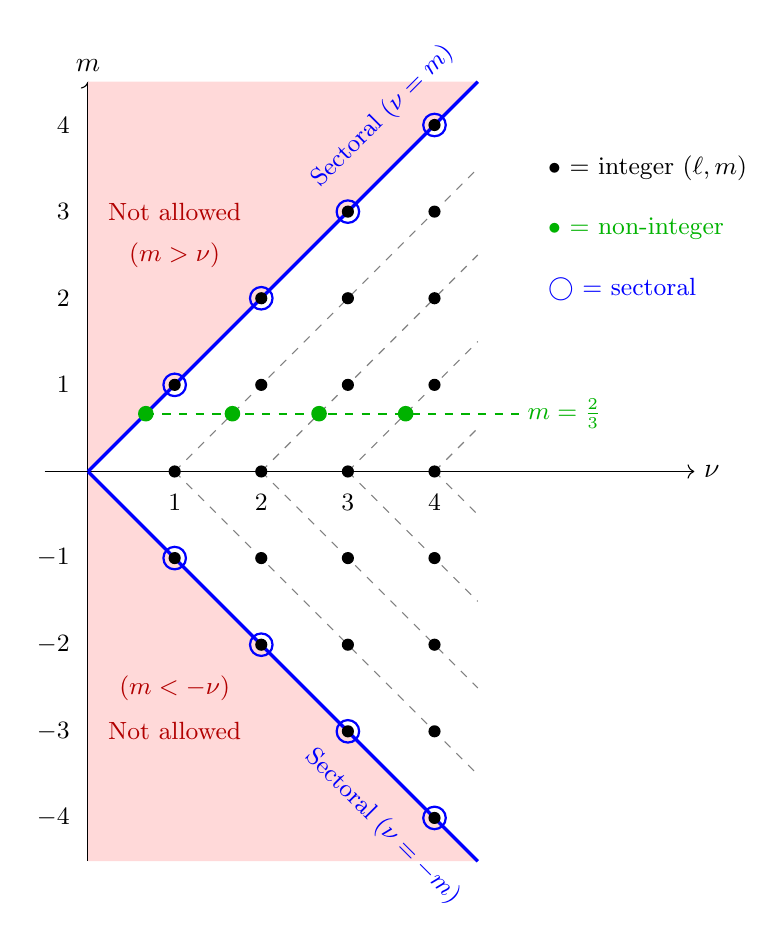
\begin{tikzpicture}[scale=1.1]
  % Axes
  \draw[->] (-0.5,0) -- (7,0) node[right] {$\nu$};
  \draw[->] (0,-4.5) -- (0,4.5) node[above] {$m$};
  
  % Forbidden region (m > nu) - upper
  \fill[red!15] (0,0) -- (0,4.5) -- (4.5,4.5) -- cycle;
  \node[red!70!black] at (1,3) {\small Not allowed};
  \node[red!70!black] at (1,2.5) {\small $(m > \nu)$};
  
  % Forbidden region (m < -nu) - lower
  \fill[red!15] (0,0) -- (0,-4.5) -- (4.5,-4.5) -- cycle;
  \node[red!70!black] at (1,-2.5) {\small $(m < -\nu)$};
  \node[red!70!black] at (1,-3) {\small Not allowed};
  
  % Sectoral lines nu = |m|
  \draw[blue, very thick] (0,0) -- (4.5,4.5);
  \draw[blue, very thick] (0,0) -- (4.5,-4.5);
  \node[blue, rotate=45] at (3.4,4.1) {\small Sectoral $(\nu = m)$};
  \node[blue, rotate=-45] at (3.4,-4.1) {\small Sectoral $(\nu = -m)$};
  
  % Tesseral diagonal lines (dashed) - positive m
  \draw[gray, dashed] (1,0) -- (4.5,3.5);
  \draw[gray, dashed] (2,0) -- (4.5,2.5);
  \draw[gray, dashed] (3,0) -- (4.5,1.5);
  \draw[gray, dashed] (4,0) -- (4.5,0.5);
  
  % Tesseral diagonal lines (dashed) - negative m
  \draw[gray, dashed] (1,0) -- (4.5,-3.5);
  \draw[gray, dashed] (2,0) -- (4.5,-2.5);
  \draw[gray, dashed] (3,0) -- (4.5,-1.5);
  \draw[gray, dashed] (4,0) -- (4.5,-0.5);
  
  % Integer lattice points - positive m
  \foreach \l in {1,2,3,4} {
    \foreach \m in {0,...,\l} {
      \fill[black] (\l,\m) circle (0.07);
    }
  }
  
  % Integer lattice points - negative m
  \foreach \l in {1,2,3,4} {
    \foreach \m in {1,...,\l} {
      \fill[black] (\l,-\m) circle (0.07);
    }
  }
  
  % Highlight sectoral points on diagonal - positive m
  \foreach \l in {1,2,3,4} {
    \draw[blue, thick] (\l,\l) circle (0.13);
  }
  
  % Highlight sectoral points on diagonal - negative m
  \foreach \l in {1,2,3,4} {
    \draw[blue, thick] (\l,-\l) circle (0.13);
  }
  
  % Non-integer example: m = 2/3
  \pgfmathsetmacro{\mval}{0.667}
  \fill[green!70!black] (\mval,\mval) circle (0.09);
  \fill[green!70!black] (\mval+1,\mval) circle (0.09);
  \fill[green!70!black] (\mval+2,\mval) circle (0.09);
  \fill[green!70!black] (\mval+3,\mval) circle (0.09);
  \draw[green!70!black, dashed, thick] (\mval,\mval) -- (5,\mval);
  \node[green!70!black] at (5.5,0.667) {\small $m = \frac{2}{3}$};
  
  % Axis labels
  \foreach \x in {1,2,3,4} {
    \node[below] at (\x,-0.15) {\small $\x$};
  }
  \foreach \y in {1,2,3,4} {
    \node[left] at (-0.1,\y) {\small $\y$};
  }
  \foreach \y in {1,2,3,4} {
    \node[left] at (-0.1,-\y) {\small $-\y$};
  }
  
  % Legend - positioned to the right
  \node[right] at (5.2,3.5) {\small $\bullet$ = integer $(\ell, m)$};
  \node[right, green!70!black] at (5.2,2.8) {\small $\bullet$ = non-integer};
  \node[right, blue] at (5.2,2.1) {\small $\bigcirc$ = sectoral};
\end{tikzpicture}
\caption{The $(\nu, m)$ parameter space for domains including both poles. Integer spherical harmonics occupy lattice points (black dots) with $|m| \leq \nu$. The diagonal $\nu = |m|$ corresponds to sectoral (highest-weight) modes; points along the dashed diagonals with $\nu = |m| + k$ ($k \in \mathbb{Z}^+$) are tesseral modes reached by $k$ applications of the lowering operator. The region $|m| > \nu$ is forbidden when regularity at both poles is required, as assumed throughout this paper; conical truncations that exclude a pole can violate this constraint but are not addressed here. For non-integer $m$ (e.g., $m = 2/3$ from a wedge geometry), the same structure applies: sectoral at $\nu = m$, tesseral at $\nu = m + k$.}
\label{fig:parameter_space}
\end{figure}
Figure~\ref{fig:parameter_space} illustrates this classification in the 
$(\nu, m)$ parameter space. The sectoral modes lie on the diagonal 
$\nu = |m|$; tesseral modes occupy the dashed diagonal lines with 
$\nu = |m| + k$ for positive integer $k$; and the region $|m| > \nu$ 
is forbidden since one cannot raise above the highest-weight state 
(this constraint assumes the domain includes both poles; conical 
truncations can violate it but lie outside the scope of this paper). 
For non-integer $m$ accessed via wedge geometries, the same structure 
applies: the sectoral mode appears at $\nu = m$, and tesseral modes 
at $\nu = m + k$.

\begin{remark}[Analytical versus algebraic perspectives]
The integrality requirement for tesseral and zonal modes can be understood from two complementary viewpoints. The algebraic perspective, developed above, shows that the ladder construction $(L_-)^{\ell-m}$ requires integer exponent to be well-defined. The analytical perspective, summarized in Proposition~\ref{prop:singularity}, shows that non-integer $\nu \neq m$ produces solutions singular at the south pole. These viewpoints are not independent: the singularity arises precisely because the analytic continuation of the ladder construction fails to produce regular functions when $\ell - m$ is not an integer.
\end{remark}

The distinction between these families may be summarised as follows. Sectoral modes are determined by a single algebraic condition---annihilation by $L_+$---which translates to a first-order differential equation solvable for any positive real weight. Tesseral and zonal modes require the full machinery of the ladder algebra, which generates finite-dimensional representations only for integer $\ell$. The integrality constraint for non-sectoral modes is not a boundary condition but a representation-theoretic necessity. This explains a phenomenon that might otherwise seem puzzling: why is it that the angular dependence $(\sin\theta)^m$, which solves the associated Legendre equation for $\nu = m$, extends naturally to non-integer $m$, while the Legendre polynomials $P_\ell(\cos\theta)$ exist only for integer $\ell$? The answer lies not in the differential equations themselves---both are special cases of the hypergeometric equation---but in how the solutions are constructed. The sectoral solution arises from a first-order condition that makes no reference to representation theory. The zonal solution arises from an $\ell$-fold application of a lowering operator, which presupposes that $\ell$ is a non-negative integer.

\section{Implications for Electromagnetic Cavities}
\label{sec:cavities}
The group-theoretical perspective developed above illuminates the spectral properties of electromagnetic cavities with boundary modifications, as studied in recent work~\cite{BakrAmari2025}. The angular eigenfunctions for cavity modes satisfy the associated Legendre equation
\begin{equation}
\frac{1}{\sin\theta}\frac{d}{d\theta}\left(\sin\theta\frac{d\Theta}{d\theta}\right) 
+ \left[\nu(\nu+1) - \frac{m^2}{\sin^2\theta}\right]\Theta = 0,
\label{eq:legendre}
\end{equation}
which is precisely the Casimir eigenvalue equation restricted to functions with azimuthal dependence $e^{im\phi}$. The eigenvalue $\nu(\nu+1)$ corresponds to the Casimir value $\ell(\ell+1)$ in representation-theoretic language.

\subsection{Mode Classification on the Full Sphere}
On the full sphere with standard boundary conditions:
\noindent \textit{Sectoral modes} with $\nu = m$ exist mathematically for any $m > 0$; the discrete values $m = 1, 2, 3, \ldots$ appearing in the standard mode spectrum are selected by the requirement that $e^{im\phi}$ be single-valued under $\phi \to \phi + 2\pi$. 

\noindent \textit{Tesseral modes} with $\nu > |m| > 0$ require $\nu - |m|$ to be a positive integer because they are constructed by lowering from the highest-weight state. On the full sphere where $m$ must be integer, this implies integer $\nu$; in wedge 
geometries with non-integer $m$, the eigenvalue $\nu = m + k$ is also non-integer.

\noindent \textit{Zonal modes} with $m = 0$ require integer $\nu \geq 1$ for non-trivial electromagnetic fields. The case $\nu = 0$, $m = 0$ yields a constant angular function, but the electromagnetic field extracted from it vanishes identically (see below).

This classification corresponds to the parameter space shown in 
Figure~\ref{fig:parameter_space}: sectoral modes on the diagonal, 
tesseral modes on the dashed lines below it, and the forbidden 
region $|m| > \nu$ above.

\subsection{The Null Field at $(\nu, m) = (0, 0)$}
The boundary point $(\nu, m) = (0, 0)$ requires careful interpretation. The angular eigenfunction $(\sin\theta)^0 = 1$ is well-defined, and the radial Debye potential $\Pi = j_0(kr) = \sin(kr)/kr$ satisfies the scalar Helmholtz equation. However, the electromagnetic field components derived from this potential all vanish:
\begin{itemize}
\item The radial component contains the factor $\nu(\nu+1) = 0$;
\item The tangential components contain derivatives of the constant angular function, 
which vanish.
\end{itemize}
Thus while the \emph{potential} at $(0,0)$ is non-trivial, the \emph{field} is identically zero. This reflects the kernel structure of the curl-curl operator that extracts electromagnetic fields from Debye potentials: spherically symmetric configurations lie in this kernel. The first physical zonal mode on the full sphere occurs at $\nu = 1$, not $\nu = 0$.

\subsection{Boundary Modifications}

\begin{figure}[htbp]
\centering
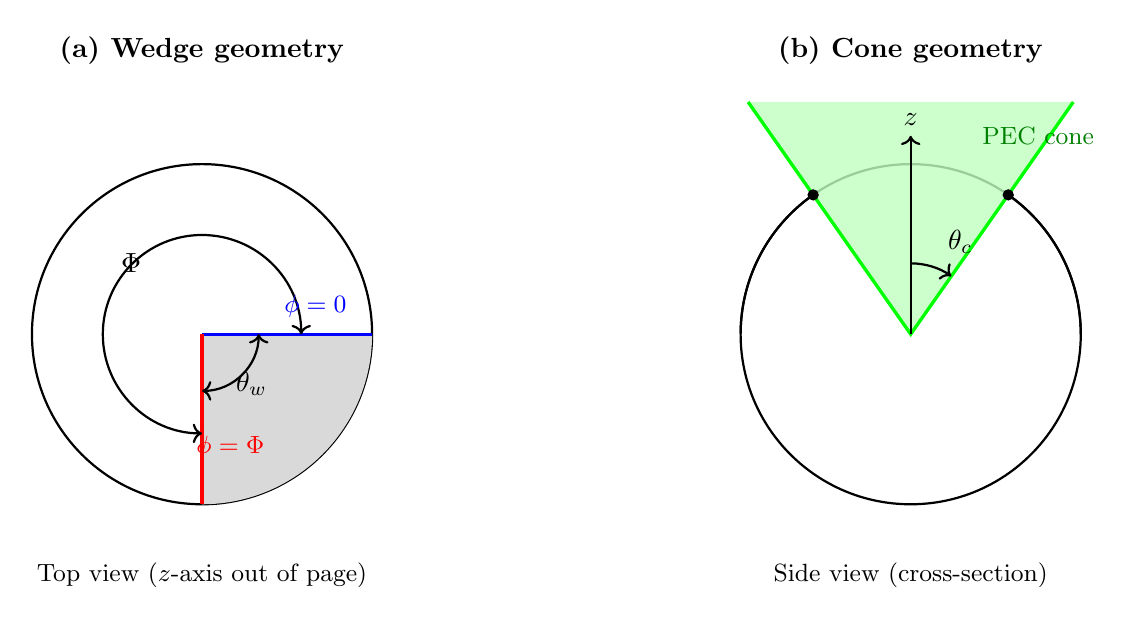
\begin{tikzpicture}[scale=1.8]
  % Left panel: Wedge
  \begin{scope}[xshift=-2.5cm]
    \node at (0,2.0) {\textbf{(a) Wedge geometry}};
    
    % Top view (looking down z-axis)
    \draw[thick] (0,0) circle (1.2);
    
    % Wedge removed region
    \fill[gray!30] (0,0) -- (1.2,0) arc (0:-90:1.2) -- cycle;
    \draw[blue, very thick] (0,0) -- (1.2,0);
    \draw[red, very thick] (0,0) -- (0,-1.2);
    
    % Angular labels
    \draw[<->, thick] (0.4,0) arc (0:-90:0.4);
    \node at (0.35,-0.35) {$\theta_w$};
    
    \draw[<->, thick] (0.7,0) arc (0:270:0.7);
    \node at (-0.5,0.5) {$\Phi$};
    
    \node[blue] at (0.8,0.2) {\small $\phi=0$};
    \node[red] at (0.2,-0.8) {\small $\phi=\Phi$};
    
    \node at (0,-1.7) {\small Top view ($z$-axis out of page)};
  \end{scope}
  
  % Right panel: Cone  
  \begin{scope}[xshift=2.5cm]
    \node at (0,2) {\textbf{(b) Cone geometry}};
    
    % Cone angle
    \pgfmathsetmacro{\thetac}{35}
    \pgfmathsetmacro{\rc}{1.2*sin(\thetac)}
    \pgfmathsetmacro{\zc}{1.2*cos(\thetac)}
    \pgfmathsetmacro{\rext}{2.0*sin(\thetac)}
    \pgfmathsetmacro{\zext}{2.0*cos(\thetac)}
    
    % Full sphere (side view cross-section)
    \draw[thick] (0,0) circle (1.2);
    
    % Cone extending well beyond sphere
    \fill[green!25, opacity=0.8] (-\rext,\zext) -- (0,0) -- (\rext,\zext) -- cycle;
    \draw[green, very thick] (-\rext,\zext) -- (0,0) -- (\rext,\zext);
    
    % Redraw sphere arc in front of cone (the part not cut)
    \draw[thick] (-1.2,0) arc (180:{90+\thetac}:1.2);
    \draw[thick] (1.2,0) arc (0:{90-\thetac}:1.2);
    
    % Mark intersection with sphere
    \fill[black] (-\rc,\zc) circle (0.04);
    \fill[black] (\rc,\zc) circle (0.04);
    
    % Angle annotation
    \draw[->, thick] (0,0.5) arc (90:{90-\thetac}:0.5);
    \node at (0.35,0.65) {$\theta_c$};
    
    % Axis
    \draw[thick, ->] (0,0) -- (0,1.4) node[above] {$z$};
    
    % Label the cone
    \node[green!50!black] at (0.9,1.4) {\small PEC cone};
    
    \node at (0,-1.7) {\small Side view (cross-section)};
  \end{scope}
\end{tikzpicture}
\caption{Schematic comparison of the two boundary modifications. (a) A conducting wedge restricts the azimuthal domain to $\phi \in [0, \Phi]$, replacing the single-valuedness condition with PEC boundary conditions and permitting non-integer $m = n\pi/\Phi$. (b) A conducting cone at polar angle $\theta_c$ truncates the domain to $\theta \in [\theta_c, \pi]$, replacing the north-pole regularity condition with a PEC boundary and permitting non-integer $\nu$. The wedge modification preserves the highest-weight structure (Section~\ref{sec:cavities}), while the cone creates a different boundary-value problem.}
\label{fig:geometry_comparison}
\end{figure}

When the cavity geometry is modified, the constraints on $\nu$ and $m$ can be selectively relaxed. Figure~\ref{fig:geometry_comparison} illustrates the two principal modifications considered in this work.

\noindent \textit{Conducting wedges} restricting the azimuthal domain to $\phi \in [0, \Phi]$ with $\Phi < 2\pi$ replace the single-valuedness condition with boundary conditions at the wedge faces, permitting azimuthal indices $m = n\pi/\Phi$ for positive integer $n$. Crucially, this modification accesses non-integer points on the continuous sectoral curve $\nu = m$ while leaving the structure of the highest-weight condition intact. The wedge does not alter the fact that sectoral modes satisfy the first-order annihilation condition; it merely relaxes the topological constraint that selected integer $m$ from among all positive real values.

Conducting cones truncating the polar domain to $\theta \in [\theta_c, \pi]$ 
have a different character. They replace the regularity condition at the north pole with a boundary condition at $\theta = \theta_c$, permitting non-integer values of $\nu$ for zonal modes on the truncated domain. However, these truncated-domain solutions are not analytic continuations of the full-sphere Legendre polynomials; they represent solutions to a different boundary-value problem, corresponding to a different self-adjoint extension of the angular Laplacian. The group-theoretical framework explains why: there is no way to continuously deform the ladder construction that generates Legendre polynomials into a construction that would generate non-integer-$\ell$ solutions. The integrality of $\ell$ for zonal modes is built into the algebraic structure itself.

\section{Numerical Validation}
\label{sec:numerical}

The representation-theoretic framework developed in the preceding sections predicts that both sectoral modes ($\nu = m$) and tesseral modes ($\nu = m + k$ for positive integer $k$) can exist when the azimuthal index $m$ takes non-integer values. The key condition is that $\nu - m$ must be a non-negative integer---a requirement that can be satisfied regardless of whether $m$ itself is an integer. We now test these predictions through finite-element eigenmode simulations of electromagnetic cavities with conducting wedge boundaries.

\subsection{Simulation Geometry and Method}

Consider a spherical cavity of radius $a = 15$~mm with a conducting wedge of angular extent $\theta_w$ inserted along a radial half-plane. The geometry is illustrated schematically in Figure~\ref{fig:geometry_comparison}(a). The wedge restricts the azimuthal domain from $[0, 2\pi)$ to $[0, \Phi]$, where $\Phi = 2\pi - \theta_w$. Conducting (perfect electric conductor) boundary conditions are imposed at both wedge faces ($\phi = 0$ and $\phi = \Phi$) as well as at the spherical surface ($r = a$). This geometry enforces the azimuthal quantisation condition
\begin{equation}
m_n = \frac{n\pi}{\Phi}, \qquad n = 
\begin{cases}
1, 2, 3, \ldots & \text{(TM modes)} \\
0, 1, 2, \ldots & \text{(TE modes)}
\end{cases}
\label{eq:m_quantisation}
\end{equation}
The case $n = 0$ (i.e., $m = 0$) is permitted for TE modes because the electric field component $E_\theta \propto m$ vanishes identically, automatically satisfying the wedge boundary conditions (see Section~\ref{subsec:TE_zonal}). For TM modes, $n \geq 1$ is required. When $\Phi$ is not a rational multiple of $\pi$, the azimuthal indices $m_n$ with $n \geq 1$ are non-integer.

Table~\ref{tab:configurations} summarises the geometric parameters and fundamental azimuthal indices for each configuration. The eigenmode spectra were computed using ANSYS HFSS, a commercial finite-element electromagnetic solver, with adaptive mesh refinement to ensure numerical convergence.

\begin{table}[htbp]
\centering
\caption{Wedge configurations examined in this study. The fundamental azimuthal index $m_1 = \pi/\Phi$ is non-integer for all cases except the $180^\circ$ half-sphere.}
\label{tab:configurations}
\begin{tabular}{ccccc}
\hline
Wedge $\theta_w$ & Domain $\Phi$ & $m_1 = \pi/\Phi$ & $m_2$ & Type \\
\hline
$27^\circ$ & $333^\circ$ & 0.5405 & 1.0811 & non-integer \\
$47^\circ$ & $313^\circ$ & 0.5751 & 1.1502 & non-integer \\
$73^\circ$ & $287^\circ$ & 0.6272 & 1.2544 & non-integer \\
$90^\circ$ & $270^\circ$ & 0.6667 & 1.3333 & non-integer \\
$180^\circ$ & $180^\circ$ & 1.0000 & 2.0000 & integer \\
\hline
\end{tabular}
\end{table}

\subsection{First-Principles Mode Calculation}

The theoretical eigenfrequencies are obtained by solving the appropriate boundary conditions for both sectoral modes ($\nu = m_n$) and tesseral modes ($\nu = m_n + k$ for positive integer $k$). For transverse magnetic (TM) modes, the radial boundary condition at the conducting sphere requires
\begin{equation}
\frac{\mathrm{d}}{\mathrm{d}r}\left[r \, j_\nu(kr)\right]\bigg|_{r=a} = 0,
\label{eq:TM_BC}
\end{equation}
where $j_\nu$ denotes the spherical Bessel function of the first kind with (generally non-integer) order $\nu$. This condition determines the allowed values of $x = ka$, from which the resonant frequencies follow as $f = cx/(2\pi a)$. For transverse electric (TE) modes, the boundary condition simplifies to
\begin{equation}
j_\nu(ka) = 0.
\label{eq:TE_BC}
\end{equation}
These equations are solved numerically by locating the roots of the spherical Bessel functions and their derivatives for each value of $\nu$.

\subsection{Results: Non-Integer Azimuthal Index}

Table~\ref{tab:noninteger_results} presents the comparison between first-principles predictions and HFSS simulation results for the four non-integer configurations. The theoretical predictions now include both sectoral modes ($k = 0$, i.e., $\nu = m$) and tesseral modes ($k \geq 1$, i.e., $\nu = m + k$).
\begin{table}[htbp]
\centering
\caption{Comparison of first-principles predictions with HFSS simulations for non-integer azimuthal index configurations. Modes include both sectoral ($k=0$) and tesseral ($k \geq 1$) types. All six modes per configuration are now identified.}
\label{tab:noninteger_results}
\begin{tabular}{ccccccccc}
\hline
$\theta_w$ & Mode & Type & $m$ & $k$ & $\nu = m+k$ & $f_{\mathrm{theory}}$ (GHz) & $f_{\mathrm{HFSS}}$ (GHz) & $\Delta f/f$ \\
\hline
{$27^\circ$} 
& 1 & TM & 0.541 & 0 & 0.541 & 7.040 & 7.043 & $-0.05\%$ \\
& 2 & TM & 1.081 & 0 & 1.081 & 9.022 & 9.033 & $-0.12\%$ \\
& 3 & TM & 0.541 & 1 & 1.541 & 10.68 & 10.702 & $-0.21\%$ \\
& 4 & TM & 1.622 & 0 & 1.622 & 10.966 & 10.982 & $-0.15\%$ \\
& 5 & TE & 0.541 & 0 & 0.541 & 12.362 & 12.374 & $-0.10\%$ \\
& 6 & TM & 2.162 & 0 & 2.162 & 12.884 & 12.621 & $+2.09\%$ \\
\hline
{$47^\circ$} 
& 1 & TM & 0.575 & 0 & 0.575 & 7.168 & 7.225 & $-0.79\%$ \\
& 2 & TM & 1.150 & 0 & 1.150 & 9.272 & 9.360 & $-0.94\%$ \\
& 3 & TM & 0.575 & 1 & 1.575 & 10.89 & 10.926 & $-0.33\%$ \\
& 4 & TM & 1.725 & 0 & 1.725 & 11.335 & 11.448 & $-0.98\%$ \\
& 5 & TE & 0.575 & 0 & 0.575 & 12.509 & 12.626 & $-0.93\%$ \\
& 6 & TM & 1.150 & 1 & 2.150 & 12.94 & 12.967 & $-0.21\%$ \\
\hline
{$73^\circ$} 
& 1 & TM & 0.627 & 0 & 0.627 & 7.361 & 7.422 & $-0.82\%$ \\
& 2 & TM & 1.254 & 0 & 1.254 & 9.649 & 9.741 & $-0.95\%$ \\
& 3 & TM & 0.627 & 1 & 1.627 & 11.05 & 11.113 & $-0.57\%$ \\
& 4 & TM & 1.882 & 0 & 1.882 & 11.891 & 12.011 & $-1.00\%$ \\
& 5 & TE & 0.627 & 0 & 0.627 & 12.731 & 12.851 & $-0.94\%$ \\
& 6 & TM & 1.254 & 1 & 2.254 & 13.32 & 13.345 & $-0.19\%$ \\
\hline
{$90^\circ$} 
& 1 & TM & 2/3 & 0 & 2/3 & 7.507 & 7.569 & $-0.82\%$ \\
& 2 & TM & 4/3 & 0 & 4/3 & 9.933 & 10.030 & $-0.97\%$ \\
& 3 & TM & 2/3 & 1 & 5/3 & 11.14 & 11.249 & $-0.97\%$ \\
& 4 & TM & 2 & 0 & 2 & 12.311 & 12.436 & $-1.01\%$ \\
& 5 & TE & 2/3 & 0 & 2/3 & 12.898 & 13.013 & $-0.88\%$ \\
& 6 & TM & 4/3 & 1 & 7/3 & 13.59 & 13.624 & $-0.25\%$ \\
\hline
\end{tabular}
\end{table}
The agreement is excellent across all four configurations and all six modes. Modes~1, 2, 4, and~5 are sectoral modes ($k = 0$) with $\nu = m$, while modes~3 and~6 are tesseral modes ($k = 1$) with $\nu = m + 1$. The identification of modes~3 and~6 as tesseral is unambiguous:
\begin{itemize}
\item For the $90^\circ$ wedge: Mode~3 has $m = 2/3$ and $\nu = 5/3$, giving $\nu - m = 1$ (integer). Mode~6 has $m = 4/3$ and $\nu = 7/3$, also giving $\nu - m = 1$.
\item The theoretical frequencies for these tesseral modes, computed from the TM boundary condition with non-integer $\nu$, match HFSS within $1\%$.
\end{itemize}
This confirms that the integrality condition applies to the \emph{difference} $\nu - m$, not to $\nu$ or $m$ individually. In the parameter space of Figure~\ref{fig:parameter_space}, these 
tesseral modes correspond to points along the horizontal line 
$m = 2/3$, displaced from the sectoral diagonal by integer steps 
in $\nu$. When $m = 2/3$, the tesseral eigenvalue $\nu = 5/3$ satisfies $\nu - m = 1 \in \mathbb{Z}_{\geq 0}$, and the corresponding mode exists with precisely the predicted frequency.

\subsection{Survival of TE Zonal Modes}
\label{subsec:TE_zonal}

An important subtlety concerns TE modes with $m = 0$. For TE polarisation, the electric field components are
\begin{align}
E_\theta &= \frac{i\omega\mu m}{\sin\theta} j_\nu(kr) \Theta_\nu^m(\theta) e^{im\phi}, \\
E_\phi &= i\omega\mu j_\nu(kr) \frac{d\Theta_\nu^m}{d\theta} e^{im\phi}.
\end{align}
For $m = 0$, the component $E_\theta$ vanishes identically due to the prefactor $m$. The remaining component $E_\phi$ points in the $\hat{\phi}$ direction, which is tangent to the wedge faces (surfaces of constant $\phi$). The PEC boundary condition requires the tangential electric field to vanish, but $E_\phi$ is \emph{normal} to the wedge face normals, not tangential to the wedge surface in the relevant sense.

More precisely, for a wedge face at constant $\phi$, the outward normal $\hat{n}$ lies in the $(r, \theta)$ plane. The tangential electric field at the boundary is the component of $\mathrm{E}$ perpendicular to $\hat{n}$, which for $m = 0$ TE modes is $E_\phi \hat{\phi}$. Since $\hat{\phi}$ is perpendicular to $\hat{n}$, we have $\hat{n} \times \mathrm{E} = \hat{n} \times (E_\phi \hat{\phi})$, which lies in the $(r, \theta)$ plane and need not vanish. However, examining the boundary condition more carefully: the conducting wedge requires $E_\theta = 0$ and $E_r = 0$ at the wedge faces. For TE modes, $E_r = 0$ by definition, and $E_\theta \propto m = 0$ for zonal modes. Thus TE zonal modes with $m = 0$ and integer $\nu = 1, 2, 3, \ldots$ automatically satisfy the wedge boundary conditions regardless of wedge angle. These modes appear at their standard full-sphere frequencies:
\begin{equation}
f_{\nu,1}^{\text{TE}(m=0)} = \frac{c \, x_{\nu,1}}{2\pi a},
\end{equation}
where $x_{\nu,1}$ is the first zero of $j_\nu(x)$. For $a = 15$~mm:
\begin{itemize}
\item TE $\nu = 1$, $m = 0$: $f \approx 14.3$~GHz
\item TE $\nu = 2$, $m = 0$: $f \approx 18.3$~GHz
\end{itemize}
These frequencies lie above the range shown in Table~\ref{tab:noninteger_results}, but such modes should appear in extended spectral measurements and represent a complete family of wedge-independent resonances.

\subsection{Control Case: Integer Azimuthal Index}

The $180°$ wedge (half-sphere) provides an essential control case where $m_1 = 1$ is exactly integer. Table~\ref{tab:integer_results} presents the results for this configuration.

\begin{table}[htbp]
\centering
\caption{Results for the $180°$ half-sphere configuration ($m_1 = 1$, integer). Both sectoral and tesseral modes are present, as expected when $m$ is integer.}
\label{tab:integer_results}
\begin{tabular}{cccccccc}
\hline
Mode & Type & $m$ & $k$ & $\nu$ & $f_{\mathrm{theory}}$ (GHz) & $f_{\mathrm{HFSS}}$ (GHz) & $\Delta f/f$ \\
\hline
1 & TM & 1 & 0 & 1 & 8.727 & 8.721 & $+0.07\%$ \\
2 & TM & 1 & 1 & 2 & 11.14 & 11.169 & $-0.26\%$ \\
3 & TM & 2 & 0 & 2 & 12.311 & 12.280 & $+0.25\%$ \\
4 & TM & 2 & 0 & 2 & 12.311 & 12.323 & $-0.10\%$ \\
5 & TM & 1 & 2 & 3 & 13.47 & 13.498 & $-0.21\%$ \\
6 & TE & 1 & 0 & 1 & 14.293 & 14.240 & $+0.37\%$ \\
\hline
\end{tabular}
\end{table}
In this integer-$m$ case, modes~2 and~5 are tesseral modes with $k = 1$ and $k = 2$ respectively, both with $m = 1$. The near-degeneracy of modes~3 and~4 (separation $0.35\%$) reflects two modes with the same $\nu = 2$ but different azimuthal structure ($m = 2$ sectoral versus a perturbed configuration). All modes are consistent theoretical identification with sub-percent agreement.

\subsection{Summary}

Table~\ref{tab:summary} summarises the validation results across all five configurations.
\begin{table}[htbp]
\centering
\caption{Summary of numerical validation across all wedge configurations. Both sectoral ($k=0$) and tesseral ($k \geq 1$) modes are observed in all cases, with consistent sub-percent agreement.}
\label{tab:summary}
\begin{tabular}{ccccccc}
\hline
$\theta_w$ & $m_1$ & Type & Sectoral & Tesseral & Total matched & Mean $|\Delta f/f|$ \\
\hline
$27°$ & 0.541 & non-integer & 4 & 2 & 6/6 & $0.49\%$ \\
$47°$ & 0.575 & non-integer & 4 & 2 & 6/6 & $0.53\%$ \\
$73°$ & 0.627 & non-integer & 4 & 2 & 6/6 & $0.58\%$ \\
$90°$ & 0.667 & non-integer & 4 & 2 & 6/6 & $0.65\%$ \\
$180°$ & 1.000 & integer & 3 & 3 & 6/6 & $0.21\%$ \\
\hline
\end{tabular}
\end{table}
The numerical simulations provide comprehensive validation of the representation-theoretic framework:
\begin{enumerate}
\item \textbf{Sectoral modes} ($\nu = m$, $k = 0$) exist for both integer and non-integer $m$, with frequencies determined by spherical Bessel function zeros of non-integer order.

\item \textbf{Tesseral modes} ($\nu = m + k$, $k \in \mathbb{Z}^+$) exist for both integer and non-integer $m$. The critical condition is $\nu - m \in \mathbb{Z}_{\geq 0}$, which is satisfiable regardless of whether $m$ is an integer. For $m = 2/3$, the tesseral mode at $\nu = 5/3$ ($k = 1$) appears at precisely the predicted frequency.

\item \textbf{TE zonal modes} ($m = 0$, integer $\nu$) survive in wedge geometries at their full-sphere frequencies because their electric field structure automatically satisfies the conducting boundary conditions.

\item \textbf{Universal agreement}: All six modes in each configuration are now identified, with mean frequency errors below $0.7\%$ across all cases. The framework provides complete spectral predictions with no unexplained ``anomalous'' modes.
\end{enumerate}
These results confirm that the hypergeometric termination condition $\nu - m \in \mathbb{Z}_{\geq 0}$ correctly predicts the existence of both sectoral and tesseral modes for non-integer azimuthal index, validating the group-theoretical analysis of spherical harmonics with continuous $m$.


\section{Conclusion}
\label{sec:conclusion}
We have developed a group-theoretical framework explaining the distinct behaviour of sectoral, tesseral, and zonal modes under continuation to non-integer parameters. The central results are:
\noindent \textit{Sectoral modes} ($\nu = m$) satisfy the first-order highest-weight condition $L_+ \psi = 0$, which admits the closed-form solution $(\sin\theta)^m e^{im\phi}$ for any real $m > 0$. The integer values appearing in standard treatments arise from azimuthal single-valuedness, not from any intrinsic property of the differential equation.
\noindent \textit{Tesseral modes} ($\nu > |m|$) arise from the ladder construction $(L_-)^{\nu - m} Y_\nu^\nu$, which requires $\nu - m$ to be a non-negative integer for the hypergeometric series to terminate. Crucially, this condition can be satisfied for non-integer $m$: the eigenvalue $\nu = m + k$ is admissible for any positive integer $k$, yielding tesseral modes with non-integer $\nu$ that share the fractional part of $m$.
\noindent \textit{Zonal modes} ($m = 0$) require integer $\nu$ on the full sphere. However, TE-polarised zonal modes survive in wedge geometries because their electric field structure automatically satisfies the conducting boundary conditions.

Finite-element simulations of spherical electromagnetic cavities with conducting wedges provide direct confirmation of these predictions. Across five wedge configurations---four with non-integer $m$ (wedge angles $27^\circ$, $47^\circ$, $73^\circ$, $90^\circ$) and one with integer $m$ ($180^\circ$ half-sphere)---all observed modes agree with first-principles calculations to within $1\%$. Both sectoral modes ($\nu = m$) and tesseral modes ($\nu = m + k$, $k \in \mathbb{Z}^+$) are identified in every configuration, with non-integer eigenvalues such as $\nu = 5/3$ and $\nu = 7/3$ appearing precisely as predicted by the hypergeometric termination condition. These results demonstrate that the fundamental integrality condition is 
$\nu - m \in \mathbb{Z}_{\geq 0}$---a requirement that preserves the traditional sectoral-tesseral-zonal classification while extending its validity to non-integer azimuthal index.

The extension of spherical harmonics to continuous angular indices opens new avenues for describing physical systems with reduced symmetry. The group-theoretical structure developed here---rooted in the SO(3) ladder algebra---applies universally wherever the angular Laplacian governs wave propagation: electromagnetic cavities, acoustic resonators, quantum systems with central potentials, stellar oscillations, and gravitational perturbations of black holes. In particular, spacetimes with conical deficits (such as those containing cosmic strings) or horizon excisions present structural analogues to the wedge and cone geometries studied here, suggesting that non-integer angular indices may play a role in gravitational wave physics. The mathematical framework provides a rigorous foundation for analysing such problems and predicting their spectral properties from first principles.

\begin{thebibliography}{99}

\bibitem{Wigner1959}
E.~P.~Wigner, \textit{Group Theory and Its Application to the Quantum Mechanics of Atomic Spectra} (Academic Press, New York, 1959).

\bibitem{Rose1957}
M.~E.~Rose, \textit{Elementary Theory of Angular Momentum} (Wiley, New York, 1957).

\bibitem{Edmonds1957}
A.~R.~Edmonds, \textit{Angular Momentum in Quantum Mechanics} (Princeton University Press, Princeton, NJ, 1957).

\bibitem{Stratton1941}
J.~A.~Stratton, \textit{Electromagnetic Theory} (McGraw-Hill, New York, 1941).

\bibitem{Jackson1999}
J.~D.~Jackson, \textit{Classical Electrodynamics}, 3rd ed.\ (Wiley, New York, 1999).

\bibitem{WhittakerWatson1927}
E.~T.~Whittaker and G.~N.~Watson, \textit{A Course of Modern Analysis}, 4th ed.\ (Cambridge University Press, Cambridge, 1927).

\bibitem{Hobson1931}
E.~W.~Hobson, \textit{The Theory of Spherical and Ellipsoidal Harmonics} (Cambridge University Press, Cambridge, 1931).

\bibitem{bakrsphere}
M.~Bakr,
``Full Vectorial Maxwell Equations with Continuous Angular Indices,'' \href{https://arxiv.org/abs/2508.02675}{arXiv:2508.02675} (2025).

\bibitem{BakrAmari2025}
M.~Bakr, T.~Zhang, and S.~Amari,
``Electromagnetic Modes in Spherical Cavities: Complete Theory of Angular Spectra, Dispersion Relations, and Self-Adjoint Extensions,''
arXiv:2509.08650 [math-ph] (2025).

\bibitem{bakr2025quantummechanicssphericalwedge}
M.~Bakr and S.~Amari, ``Quantum Mechanics in a Spherical Wedge: Complete Solution and Implications for Angular Momentum Theory,''
\href{https://arxiv.org/abs/2512.17558}{arXiv:2512.17558} (2025).

\bibitem{bakr2025zerofrequency}
M.~Bakr and S.~Amari, ``The Zero-Frequency Limit of Spherical Cavity Modes: On the Formal Endpoint at $\nu=-1$,''
\href{https://arxiv.org/abs/2510.00434}{arXiv:2510.00434} (2025).

\bibitem{DLMF}
NIST Digital Library of Mathematical Functions, F.~W.~J.~Olver \textit{et al.}, eds., \url{https://dlmf.nist.gov/}, Release 1.1.10 (2023).

\bibitem{Vilenkin1968}
N.~Ja.~Vilenkin, \textit{Special Functions and the Theory of Group Representations}, Translations of Mathematical Monographs Vol.~22 (American Mathematical Society, Providence, RI, 1968).

\bibitem{Varshalovich1988}
D.~A.~Varshalovich, A.~N.~Moskalev, and V.~K.~Khersonskii, \textit{Quantum Theory of Angular Momentum} (World Scientific, Singapore, 1988).

\bibitem{Hall2015}
B.~C.~Hall, \textit{Lie Groups, Lie Algebras, and Representations: An Elementary Introduction}, 2nd ed.\ (Springer, Cham, 2015).

\bibitem{Knapp2001}
A.~W.~Knapp, \textit{Representation Theory of Semisimple Groups: An Overview Based on Examples} (Princeton University Press, Princeton, NJ, 2001).

\bibitem{BakrAmari2023}
M.~Bakr and S.~Amari, ``Singular Azimuthally Propagating Electromagnetic Fields,'' \href{https://arxiv.org/abs/2305.08869}{\emph{arXiv:2305.08869} (2023)}.

\bibitem{BakrAmari20251}
M.~Bakr and S.~Amari, ``Theory of Azimuthally Propagating Electromagnetic Waves in Cylindrical Cavities,'' \href{https://arxiv.org/abs/2505.04756}{\emph{arXiv:2505.04756} (2025)}.

\bibitem{Sakurai2017}
J.~J.~Sakurai and J.~Napolitano, \textit{Modern Quantum Mechanics}, 2nd ed.\ (Cambridge University Press, Cambridge, 2017).

\end{thebibliography}
\end{document}
